\documentclass[12pt]{article}
%%%%%%%%%%%%%%%%%% General packages
\usepackage{amssymb,amsmath,amsfonts,eurosym,ulem,graphicx,
	caption,color,setspace,sectsty,comment,footmisc,
	pdflscape,subcaption,array, multicol,multirow,tikz, bm,
        booktabs, rotating, titling, threeparttable}
\usepackage[section]{placeins}
%%%%%%%%%%%%%%%%%%% Encoding
\usepackage[utf8]{inputenc}
\DeclareUnicodeCharacter{03C4}{\ensuremath{\tau}}
\DeclareUnicodeCharacter{0394}{\ensuremath{\Delta}}
%%%%%%%%%%%%%%%%%% Margins and Spacing
\usepackage[left=1.0in,right=1.0in,top=1in,bottom=1in]{geometry}
\usepackage{indentfirst}
%%%%%%%%%%%%%%%%%% References
\usepackage[sort]{natbib}
\bibliographystyle{econ}
%%%%%%%%%%%%%%%%%% Links
\usepackage[colorlinks=true, allcolors=blue]{hyperref}
\urlstyle{same} %makes url the same font as text, not courier default
\newcommand{\doi}[1]{\url{#1}}
%%%%%%%%%%%%%%%%%% tikz/diagrams
\usetikzlibrary{arrows,shapes,positioning,intersections,calc}
%%%%%%%%%%%%%%%%%% table formatting
\newcolumntype{L}[1]{>{\raggedright\arraybackslash}p{#1}}
\newcolumntype{C}[1]{>{\centering\arraybackslash}p{#1}}
\newcolumntype{R}[1]{>{\raggedleft\arraybackslash}p{#1}}
\normalem
\makeatother
%%%%%%%%%%%%%%%%%% Float placement
\setcounter{topnumber}{3}
\setcounter{bottomnumber}{2}
\setcounter{totalnumber}{5}
\renewcommand{\topfraction}{0.9}
\renewcommand{\bottomfraction}{0.8}
\renewcommand{\textfraction}{0.07}
\renewcommand{\floatpagefraction}{0.8}
\renewcommand{\dbltopfraction}{0.9}
\renewcommand{\dblfloatpagefraction}{0.8}
\setlength{\textfloatsep}{12pt plus 2pt minus 4pt}
\setlength{\floatsep}{10pt plus 2pt minus 2pt}
\setlength{\intextsep}{10pt plus 2pt minus 2pt}
\AtBeginEnvironment{table}{\singlespacing\footnotesize\setlength{\tabcolsep}{4pt}\renewcommand{\arraystretch}{0.95}}
\AtBeginEnvironment{figure}{\singlespacing}
%%%%%%%%%%%%%%%%%% Autoreference names
\renewcommand{\sectionautorefname}{Section}
\renewcommand{\subsectionautorefname}{Section}
\renewcommand{\figureautorefname}{Figure}
\renewcommand{\tableautorefname}{Table}
% equation numbering start at 1
\newcommand\numberthis{\addtocounter{equation}{1}\tag{\theequation}}
%%%%%%%%%%%%%%%%%% Theorem Names
\newtheorem{prop}{Proposition}
\newtheorem{definition}{Definition}
\newtheorem{lemma}{Lemma}
\newtheorem{corollary}{Corollary}
\newtheorem{result}{Result}
\newtheorem{assumption}{Assumption}
\newtheorem{theorem}{Theorem}

%%%%%%%%%%%%%%%%%% Title Information
%title page single spacing
\setstretch{1}
%subtitle command
\newcommand{\subtitle}[1]{\posttitle{\par\end{center}\begin{center}\large#1\end{center}\vskip0.5em}}

\title{Flood Exposure and Asset Repricing: Evidence from FEMA LOMRs and ZIP-Code Home Values}
\subtitle{Dartmouth College\\Topics in Money and Finance}
\author{Cameron Keith\thanks{I thank Professor Apoorv Gupta, Professor of Economics at Dartmouth College, for his guidance and helpful comments on this project. Claude Opus 4.6 was used to assist with code development as well as grammar and spelling checks. All analysis, interpretation, and errors are my own. \newline Email: \href{mailto:cameron.s.keith.26@dartmouth.edu}{cameron.s.keith.26@dartmouth.edu}.}}
\date{\today}

\begin{document}

\maketitle

\begin{abstract}
Do coastal housing markets reprice properties when official flood-map designations change? I study this question using FEMA Letters of Map Revision (LOMRs), localized revisions to National Flood Insurance Program (NFIP) flood maps. In a quarterly ZIP-level event study across U.S. coastal counties from 2009 to 2022, with ZIP and county-by-year fixed effects, I find that home values show near-zero response at impact but decline by about 2.8 percent four or more years after a LOMR. The decline is larger in an interaction specification with pre-treatment flood-insurance penetration. An exploratory political interaction suggests weaker repricing in Republican-leaning counties, although this comparison does not pass the pre-trend test. These findings are consistent with slow, uneven capitalization of regulatory flood-risk information rather than immediate repricing.
\end{abstract}

\doublespacing
\noindent Keywords: Flood risk; property values; FEMA; capitalization; flood insurance; event study
\\
JEL Codes: R31; Q54; G22; H84
\newpage
\setstretch{1.75}


% =============================================================================
% SECTION 1: INTRODUCTION
% =============================================================================
\section{Introduction}\label{sec:intro}

Flood risk affects housing markets through official designations and realized disasters. Federal Emergency Management Agency (FEMA) flood maps assign properties to regulatory flood-risk zones, which can affect insurance requirements, disclosure, underwriting, and buyer beliefs. The most economically salient threshold is often the Special Flood Hazard Area (SFHA), but Letters of Map Revision (LOMRs) can also matter more broadly because they update the official map that private actors use in transactions. I study whether housing markets reprice when those official designations change through FEMA LOMRs.

These stakes are large because the NFIP is both economically important and fiscally strained. As of 2025, the program covers more than 4.7 million policies with roughly \$1.3 trillion in insured value, yet it still carries \$22.5 billion in debt to the U.S. Treasury after Congress cancelled \$16 billion of NFIP debt in 2017 \citep{CRS2025_NFIPIntro,CRS2025_NFIPBorrowing}. Prior work also suggests that flood risk is not fully incorporated into housing prices: \citet{HinoBurke2021} estimate that floodplain properties are collectively overvalued by about \$44 billion and that rezoning into the floodplain is associated with roughly a 2 percent price discount.

These stakes make it economically important to understand how housing markets respond when FEMA revises the official map itself. To study that question, I construct a quarterly ZIP-level panel for coastal U.S. counties from 2009 to 2022 that combines Zillow home values with FEMA LOMRs, National Flood Insurance Program (NFIP) data, and county controls \citep{Zillow_ZHVI,FEMA_LOMR,FEMA_NFIP}. A further contribution is the construction of a linked panel that brings together home values, official flood-map revisions, insurance exposure, and local controls in one ZIP-quarter dataset. I run a staggered event study with ZIP and county-by-year fixed effects on first in-window LOMRs. I then interact treatment with pre-treatment NFIP policy penetration to analyze whether repricing is larger where mapped flood risk is already economically relevant.

Home values do not fall sharply after a LOMR. In the baseline specification, the estimated effect is close to zero at treatment and is consistent with a decline of about 2.8 percent four or more years later. The response is stronger in the continuous insurance-intensity specification, although the quartile pattern is non-monotonic. An exploratory political split also suggests weaker repricing in ZIP codes located in more Republican-leaning counties, which is suggestive of heterogeneity in attention to official flood-risk information. However, the political interaction fails the pre-trend test, so I treat that comparison as descriptive.

I study four related hypotheses. First, LOMRs are associated with lower home values. Second, if housing markets adjust with frictions, that response should emerge gradually after treatment rather than on impact. Third, if flood insurance mainly shields owners from repricing, higher pre-treatment NFIP exposure should weaken the response, while if salience dominates it should strengthen it. Fourth, if political beliefs shape attention to official flood-risk information, repricing should be weaker in more Republican counties. I test the first two with the baseline event study, the third with the intensity and insurance-outcome specifications, and the fourth with a political interaction that I treat as exploratory because its pre-trends are weaker.

The paper contributes to the flood-risk literature in three ways. First, it studies localized official map revisions rather than realized flood events, broad climate-risk disclosures, or static cross-sectional floodplain comparisons. Among prior work, \citet{ShrZipp2019} is closest in studying flood-zone remapping, while \citet{Weill2023} studies FEMA map updates as information shocks in the insurance market. Second, the staggered ZIP-level panel allows me to study the timing of capitalization after a revision becomes effective, which helps distinguish gradual repricing from an immediate market-wide reset. Third, by interacting treatment with pre-treatment NFIP penetration, I test whether the same map change carries more pricing content where flood insurance was already more financially material.

\autoref{sec:background} describes the institutional setting, \autoref{sec:literature} reviews the related literature, and \autoref{sec:data} and \autoref{sec:strategy} present the data and design. \autoref{sec:results} reports the main results, \autoref{sec:robustness} presents exploratory heterogeneity and robustness checks, \autoref{sec:discussion} discusses interpretation and limitations, and \autoref{sec:conclusion} provides areas for future research. Supporting insurance-market and subsample analyses appear in Appendix~\ref{app:tables}.


% =============================================================================
% SECTION 2: INSTITUTIONAL BACKGROUND
% =============================================================================
\section{Institutional Background}\label{sec:background}

\subsection{FEMA Flood Maps and LOMRs}\label{sec:bg_maps}

FEMA's Flood Insurance Rate Maps (FIRMs) assign properties to regulatory flood-risk zones and provide related hazard information for lenders, insurers, local governments, and buyers. Letters of Map Revision (LOMRs) update those classifications after new topographic, hydrologic, engineering, or physical information. A LOMR can move land into or out of the Special Flood Hazard Area (SFHA), revise the location of the mapped floodplain boundary, or change other map-based flood hazard information that matters for underwriting, disclosure, and insurance. The SFHA remains the most consequential threshold because federally backed mortgages in participating NFIP communities generally require flood insurance for improved structures inside that zone. However, the broader point for this paper is that LOMRs change the official map that market participants use in transactions, even when the revision does not map cleanly into a simple up-or-down SFHA crossing or follow a recent flood that has already drawn attention to the area.

\autoref{fig:lomr_example} shows a LOMR in Miami. The example makes the treatment structure concrete: the LOMR polygon overlaps two ZIP codes.

% --- Figure 1: Illustrative LOMR Map ---
\begin{figure}[!htbp]
    \centering
    \caption{Illustrative LOMR and Treated ZIP Code}
    \label{fig:lomr_example}
    \includegraphics[width=0.88\textwidth]{figures/lomr_example_florida.png}
    \caption*{\footnotesize \textit{Note: Deliberately large illustrative FEMA LOMR in Miami, Florida, chosen for visibility rather than representativeness. The shaded polygon is the revision footprint, the two ZIP codes (33165 and 33155) are treated in the event-study design, and adjacent ZIP codes remain untreated in that event window. The inset shows the location within Florida.}}
\end{figure}
\FloatBarrier

\subsection{Why LOMRs Should Affect Housing Markets}\label{sec:bg_channels}

I expect LOMRs to affect housing prices because they update the official map that market participants use to evaluate expected ownership costs. The most salient case is a revision that changes whether a property is treated as inside the SFHA, but even a boundary revision or other change in mapped flood hazard information can matter if it changes how lenders, insurers, appraisers, or buyers interpret the property. Because those actors use the official map in transactions, a LOMR can have pricing content even when no flood occurs nearby.

A lender's flood determination during underwriting may reflect the updated map, which can change insurance requirements, documentation, or the buyer's perception of risk before closing. Prices may then adjust gradually as the new information diffuses through transactions, listings, appraisals, and comparable sales rather than through an immediate market-wide reset.

% =============================================================================
% SECTION 3: RELATED LITERATURE
% =============================================================================
\section{Related Literature}\label{sec:literature}

\subsection{Flood Risk, Beliefs, and Housing Markets}\label{sec:lit_hazard}

A large literature documents that flood risk is capitalized into property values, especially after salient events. Floodplain discounts appear after hurricanes \citep{BinPolasky2004}, near-miss events \citep{HallstromSmith2005}, and severe flood experience \citep{Kousky2010}, and a meta-analysis estimates an average floodplain discount of about 4.6 percent \citep{BeltranMaddisonElliott2018}. More recent work extends those findings to broader climate-risk signals: \citet{HinoBurke2021} show that regulatory flood-risk information can affect property values even without contemporaneous damage, and \citet{BernsteinGustafsonLewis2019} document discounts for sea-level-rise exposure, although \citet{MurfinSpiegel2020} provide more skeptical evidence.

Whether risk is fully capitalized depends in part on beliefs and attention. \citet{BakkensenBarrage2022}, \citet{GibsonMullinsHill2020}, and \citet{BaldaufGarlappiYannelis2020} emphasize that capitalization varies with local climate beliefs rather than with physical exposure alone. On the disclosure side, \citet{TroyRomm2004} and \citet{Pope2008} find larger floodplain discounts under stronger disclosure rules. \citet{Weill2023} is especially close in spirit because it studies the effects of official FEMA map updates on flood-insurance take-up. I complement that literature by asking whether localized official map revisions are also capitalized into housing values.

\subsection{Difference-in-Differences with Staggered Treatment}\label{sec:lit_did}

Methodologically, \citet{GoodmanBacon2021}, \citet{SunAbraham2021}, and \citet{CallawaySantAnna2021} show why staggered TWFE event studies can be misleading when treatment timing and effects vary. I address those concerns with dynamic estimates, cautious interpretation of pooled coefficients, and heterogeneity-robust checks in \autoref{sec:robustness_checks}.

% =============================================================================
% SECTION 4: DATA
% =============================================================================
\section{Data}\label{sec:data}

\subsection{Core Panel Structure}\label{sec:data_panel}

My main estimation sample is a ZIP-by-quarter panel for U.S.\ coastal ZIP codes from 2009 to 2022. I begin with a monthly panel, because Zillow home values, NFIP insurance records, and several controls are observed at that frequency. Then, I collapse the data to quarters by averaging the monthly log values within each quarter, because the Zillow Home Value Index (ZHVI) is a three-month smoothed series and monthly observations inherit substantial serial correlation from that construction. After the sample restrictions described below, the quarterly panel contains 4,272 ZIP codes and 228,005 ZIP-quarter observations.

Those 4,272 ZIP codes include 398 single-LOMR treated ZIP codes within the estimation window, 3,711 never-treated ZIP codes, and 163 not-yet-treated ZIP codes whose first LOMR occurs after the sample window and that contribute control observations during the sample period.

\subsection{Data Sources}\label{sec:data_sources}
The primary outcome is Zillow's ZIP-level Home Value Index (ZHVI), using the all-homes (single-family residences plus condo/co-op), middle-tier, smoothed, seasonally adjusted series, which I deflate to December 2022 dollars using the Consumer Price Index for All Urban Consumers (CPI-U) \citep{FRED_CPI} and transform into $\ln(\text{real ZHVI})$ for the main specifications. Zillow's coverage determines the first major sample screen because a nontrivial share of coastal ZIP codes do not have usable home-value data over the full period.

Treatment comes from FEMA's S\_LOMR polygon layer in the National Flood Hazard Layer \citep{FEMA_LOMR}. I spatially overlay those polygons onto Census ZCTA boundaries \citep{Census_ZCTA} to identify whether a ZIP code is ever exposed to a LOMR and whether the first effective LOMR falls inside the 2009--2022 analysis window. The overlay supports the geographic-intensity extension directly. For the zoning-direction analysis, I use post-LOMR changes in SFHA share, defined as the fraction of a ZIP code's NFIP policies whose rated flood zone falls in the SFHA (A or V zones) in a given month, as a proxy for whether local flood exposure shifts upward or downward.

I merge those treatment data with OpenFEMA NFIP policy and claims records \citep{FEMA_NFIP}, which I aggregate to the ZIP-quarter level. The insurance data provide policy counts, average premiums, the share of policies rated in SFHA zones, and claims activity. Those variables serve two purposes. They measure pre-treatment exposure to flood insurance, and they also provide outcomes for the mechanism tests. From the policy counts I also construct \textit{policy intensity}, defined as the pre-LOMR average NFIP policy count divided by ZIP population, which serves as the main treatment-interaction variable in the intensity specification.

I add county-level unemployment rates from BLS Local Area Unemployment Statistics (LAUS) \citep{BLS_LAUS} as a local macro control, and I merge county presidential vote returns from the MIT Election Data and Science Lab \citep{MIT_MEDSL} to build the political heterogeneity measure. Finally, I hand-code state flood-disclosure regimes into strict and broad indicators. That combination gives me a panel that links local home values, official flood-map revisions, insurance exposure, and institutional context in a common ZIP-quarter frame.

\subsection{Sample Construction}\label{sec:data_sample}

\autoref{tab:sample_construction} summarizes the sample construction. I start from 33,782 U.S.\ ZIP codes, restrict to 5,450 ZIP codes in NOAA coastal counties, and then merge Zillow coverage, which leaves 4,836 coastal ZIP codes with usable home-value data. The LOMR--ZCTA overlay identifies 1,125 ever-treated ZIP codes in that sample, including 855 whose first observed LOMR falls inside the 2009--2022 window.

Then, I impose the event-study restrictions. First, I drop ZIP codes that were already treated before 2009 because they do not have a clean pre-period. Second, I drop ZIP codes with multiple LOMRs because overlapping revisions make event time difficult to interpret. I also winsorize $\ln(\text{real ZHVI})$ at the 1st and 99th percentiles to limit the influence of extreme observations. After these restrictions, the final regression panel contains 4,272 ZIP codes. I impose these restrictions because clean treatment timing has more value here than the additional observations they would preserve.

% --- Table 1: Sample Construction ---
\begin{table}[!htbp]
\centering
\caption{Sample Construction: From US Zip Codes to Estimation Panel}
\label{tab:sample_construction}
\begin{threeparttable}
\begin{tabular}{@{}llr@{}}
\toprule
Step & Description & Zip Codes \\
\midrule
\multicolumn{3}{@{}l}{\textit{Panel A: Geographic sample}} \\[4pt]
1 & All US zip codes & 33,782 \\
2 & Restrict to NOAA coastal counties (ocean-bordering) & 5,450 \\
3 & Merge with Zillow ZHVI (drop zips without coverage) & 4,836 \\[6pt]
\multicolumn{3}{@{}l}{\textit{Panel B: Treatment classification (within 4,836)}} \\[4pt]
  & LOMR--ZCTA spatial overlay pairs & 2,936 \\
  & Zip codes with $\geq$1 effective LOMR & 1,125 \\
  & \quad First LOMR in window (all treated zips) & 855 \\
  & \quad Single LOMR, first in window (estimation treated group) & 398 \\
  & \quad Multi-LOMR zips & 550 \\
  & \quad Already treated before 2009 & 54 \\
  & \quad First LOMR after sample window & 216 \\
  & Never-treated zip codes & 3,711 \\[6pt]
\multicolumn{3}{@{}l}{\textit{Panel C: Event-study restrictions}} \\[4pt]
4 & Drop already-treated (no clean pre-period) & $-$54 \\
  & Drop multi-LOMR (overlapping treatment timing) & $-$510 \\[2pt]
  & \textbf{Final estimation sample} & \textbf{4,272} \\
  & \quad Single-LOMR treated (in window) & 398 \\
  & \quad Not-yet-treated (first LOMR after window) & 163 \\
  & \quad Never-treated controls & 3,711 \\[2pt]
5 & Quarterly panel (after collapse) & 228,005 obs \\
\bottomrule
\end{tabular}
\begin{tablenotes}
\small
\item \textit{Notes:} Sample begins with all US zip codes from the SimpleMaps database. Step 2 restricts to zip codes within NOAA-designated coastal counties that border the ocean (excluding Alaska, Hawaii, and US territories). Step 3 drops zips lacking Zillow Home Value Index coverage. Treatment is defined by spatial overlay of FEMA LOMR polygons onto Census ZCTA boundaries. Categories in Panel B are not mutually exclusive: 40 zips are both multi-LOMR and already-treated. Panel C drops are applied sequentially; the multi-LOMR drop count (510) is net of those 40 overlapping zips already removed in the prior step (550 total multi-LOMR minus 40 overlap = 510 additional drops). Not-yet-treated zips (163) retain single LOMRs arriving after 2022 and contribute control observations during the sample period. The quarterly panel collapses monthly observations by averaging log values within each quarter.
\end{tablenotes}
\end{threeparttable}
\end{table}


\subsection{Summary Statistics}\label{sec:data_sumstats}

\autoref{tab:summary_stats} reports descriptive moments for the estimation sample. The treatment variables are highly skewed: the mean policy-intensity measure is 5.93 policies per 1,000 residents, while the median is only 0.68. Most coastal ZIP codes have limited flood-insurance exposure, while a smaller subset is much more exposed. That pattern suggests that average treatment effects may mask larger responses in places where flood insurance is already economically meaningful.

% --- Table 2: Summary Statistics ---
\begin{table}[htbp]\centering
\def\sym#1{\ifmmode^{#1}\else\(^{#1}\)\fi}
\caption{Summary Statistics: Estimation Sample (2009--2022)}
\label{tab:summary_stats}
\resizebox{\textwidth}{!}{%
\begin{tabular}{l*{1}{cccccccc}}
\hline\hline
                    &       count&        mean&          sd&         min&         p25&         p50&         p75&         max\\
\hline
\textit{Panel A: Outcomes}&            &            &            &            &            &            &            &            \\
Home Value Index (Dec 2022 \$)&     228,005&  486,214.62&  416,676.37&   32,424.71&  234,258.39&  374,152.97&  594,862.94&8,125,586.00\\
ln(Real ZHVI)       &     228,005&       12.85&        0.67&       11.36&       12.36&       12.83&       13.30&       14.56\\
ln(NFIP Policies + 1)&     228,005&        2.46&        1.80&        0.00&        0.98&        2.08&        3.71&        7.87\\
ln(NFIP Claims + 1) &     228,005&        0.11&        0.46&        0.00&        0.00&        0.00&        0.00&        8.16\\
\textit{Panel B: Treatment Variables}&            &            &            &            &            &            &            &            \\
Post-LOMR           &     228,005&        0.04&        0.19&        0.00&        0.00&        0.00&        0.00&        1.00\\
Ever Treated        &     228,005&        0.13&        0.34&        0.00&        0.00&        0.00&        0.00&        1.00\\
Policy Intensity (per 1,000)&     228,005&        5.93&       21.07&        0.00&        0.18&        0.68&        4.13&      716.99\\
Treatment Intensity (per 1,000)&     228,005&        3.60&       32.54&        0.00&        0.00&        0.00&        0.00&      944.01\\
Upzoned (into SFHA) &     228,005&        0.05&        0.21&        0.00&        0.00&        0.00&        0.00&        1.00\\
Downzoned (out of SFHA)&     228,005&        0.03&        0.18&        0.00&        0.00&        0.00&        0.00&        1.00\\
SFHA-Crossing LOMR  &     228,005&        0.08&        0.27&        0.00&        0.00&        0.00&        0.00&        1.00\\
\textit{Panel C: Controls}&            &            &            &            &            &            &            &            \\
County Unemp. Rate (\%)&     228,005&        6.47&        2.89&        1.70&        4.23&        5.80&        8.27&       29.80\\
NFIP Policies (qtr avg)&     228,005&       65.21&      164.11&        0.00&        1.67&        7.00&       39.67&    2,624.67\\
NFIP Avg Premium (\$)&     228,005&      710.36&      631.82&        0.00&      357.67&      565.67&      914.10&   19,570.33\\
NFIP Claims (qtr avg)&     228,005&        1.13&       25.22&        0.00&        0.00&        0.00&        0.00&    3,498.00\\
\textit{Panel D: Heterogeneity Measures}&            &            &            &            &            &            &            &            \\
Republican County   &     222,846&        0.50&        0.50&        0.00&        0.00&        1.00&        1.00&        1.00\\
R Two-Party Vote Share&     222,846&        0.42&        0.15&        0.06&        0.32&        0.43&        0.52&        0.89\\
Disclosure: Strict (9 states)&     228,005&        0.29&        0.45&        0.00&        0.00&        0.00&        1.00&        1.00\\
Disclosure: Broad (13 states)&     228,005&        0.61&        0.49&        0.00&        0.00&        1.00&        1.00&        1.00\\
\textit{Panel E: Sample Characteristics}&            &            &            &            &            &            &            &            \\
Zip Population      &     228,005&   19,717.91&   17,846.46&       25.00&    5,236.00&   15,229.00&   29,309.00&  109,931.00\\
Zip Pop. Density    &     228,005&    4,960.31&   11,251.76&        0.90&      225.60&    1,571.80&    4,837.00&  143,070.70\\
SFHA Zone Share     &     228,005&        0.35&        0.31&        0.00&        0.00&        0.33&        0.60&        1.00\\
\hline\hline
\end{tabular}
}% end resizebox
\end{table}

\FloatBarrier

\subsection{Balance Table}\label{sec:data_balance}

\autoref{tab:balance} compares pre-treatment means across treated and never-treated ZIP codes. Pre-treatment home values are similar, while treated ZIP codes show higher NFIP exposure (\autoref{tab:balance}), reinforcing the case for within-ZIP identification.

% --- Table 3: Balance Table ---
\begin{table}[htbp]\centering
\def\sym#1{\ifmmode^{#1}\else\(^{#1}\)\fi}
\caption{Balance Table: Pre-Treatment Characteristics}
\label{tab:balance}
\begin{tabular}{l*{1}{ccc}}
\hline\hline
                    &     Control&     Treated&  Difference         \\
\hline
Home Value (Dec 2022 \$)&  478,848.23&  474,199.50&   -4,648.73         \\
Population          &   18,542.78&   21,918.10&    3,375.32\sym{***}\\
Pop. Density (per sq mi)&    5,027.05&    3,123.25&   -1,903.80\sym{***}\\
County Unemp. Rate (\%)&        6.45&        6.80&        0.35\sym{***}\\
NFIP Policies (qtr avg)&       59.98&       84.55&       24.57\sym{***}\\
NFIP Avg Premium (\$)&      690.42&      781.76&       91.35\sym{***}\\
SFHA Zone Share     &        0.34&        0.40&        0.06\sym{***}\\
NFIP Claims (qtr avg)&        1.07&        1.35&        0.28         \\
\hline\hline
\multicolumn{4}{l}{\footnotesize Treated: zips with single LOMR during 2009-2022.}\\
\multicolumn{4}{l}{\footnotesize Control: zips with no LOMR.}\\
\multicolumn{4}{l}{\footnotesize Pre-treatment means reported for treated zips.}\\
\multicolumn{4}{l}{\footnotesize Difference = Treated $-$ Control. Welch t-test.}\\
\end{tabular}
\end{table}


% =============================================================================
% SECTION 5: EMPIRICAL STRATEGY
% =============================================================================
\section{Empirical Strategy}\label{sec:strategy}

\subsection{Baseline Event-Study Specification}\label{sec:strategy_baseline}

I estimate dynamic effects with a staggered event-study difference-in-differences design because the institutional argument in Section~\ref{sec:bg_channels} suggests gradual capitalization after a LOMR rather than an immediate one-quarter jump. The unit of observation is the ZIP-quarter. I assign treatment timing with the first effective LOMR in the 2009--2022 window, and I exclude ZIP codes with earlier treatment or multiple LOMRs because event time is otherwise difficult to interpret.

% Main estimating equation
\begin{equation}\label{eq:event_study}
    \ln(\text{Real ZHVI})_{z,t} = \alpha_z + \delta_{c(z),y(t)} + \sum_{\tau \neq -1} \beta_\tau \cdot \mathbf{1}[t - E_z = \tau] + \gamma' \mathbf{X}_{z,t} + \varepsilon_{z,t}
\end{equation}
%
\noindent In \autoref{eq:event_study}, $\alpha_z$ denotes ZIP fixed effects, $\delta_{c(z),y(t)}$ denotes county-by-year fixed effects, and $E_z$ is the effective date of the first LOMR for ZIP $z$. The coefficients of interest, $\beta_\tau$, compare treated ZIP codes at each event-time bin to the omitted year immediately before treatment, $\tau = -1$. I group event time into nine annual bins from $\tau = -4$ through $\tau = +4$: an endpoint bin for three or more years before treatment, two interior pre-treatment bins, the omitted reference year immediately before treatment, four post-treatment year bins, and an endpoint bin for four or more years after treatment. The main control vector $\mathbf{X}_{z,t}$ includes county unemployment and contemporaneous NFIP policy counts.\footnote{Including NFIP policies as a control raises a potential bad-control concern because Appendix~\ref{app:insurance} later treats policy counts as a mechanism outcome. I retain them because the event-study coefficients are nearly identical with and without NFIP controls (Column 1 vs.\ Column 2 of \autoref{tab:main_regression}).} I winsorize $\ln(\text{real ZHVI})$ at the 1st and 99th percentiles to limit the influence of outliers. I weight observations by ZIP population and cluster standard errors at the county level because treatment timing and housing-market shocks are unlikely to be independent within counties.

I prefer this specification to a single post-treatment indicator because a pooled TWFE coefficient would average together near-zero early effects and more negative late effects, hiding the timing pattern that matters for the capitalization question.

\subsection{Intensity Specification}\label{sec:strategy_intensity}

I next ask whether the same map revision has a larger price effect where flood-insurance exposure was already more salient before treatment. I expect larger responses where pre-treatment NFIP participation is higher because more households already sit near the margin where insurance costs matter. The relevant margin here is not the size of the LOMR polygon itself. It is the extent to which households in the ZIP already sat close to the insurance and disclosure margin before the map change arrived.

\begin{equation}\label{eq:intensity}
    \ln(\text{Real ZHVI})_{z,t} = \alpha_z + \delta_{c(z),y(t)} + \sum_{\tau \neq -1} \beta_\tau \cdot \mathbf{1}[t - E_z = \tau] \times \underbrace{\frac{\text{Policies}_z^{\text{pre}}}{\text{Pop}_z}}_{\text{Intensity}_z} + \gamma' \mathbf{X}_{z,t} + \varepsilon_{z,t}
\end{equation}
%
\noindent Here $\text{Intensity}_z$ is the ZIP's pre-LOMR NFIP policy count per resident. I construct it from pre-treatment policy levels so the interaction captures pre-existing exposure rather than post-treatment behavioral adjustment. That distinction matters because I want the interaction to proxy for salience, not to fold an outcome of the treatment back into the treatment itself. The coefficients in \autoref{eq:intensity} therefore show how the dynamic effect varies with baseline insurance penetration. I interpret those coefficients at realistic values of intensity, such as the sample mean or the quartiles, because an intensity value of one lies far from the center of the data.

\subsection{Identification}\label{sec:strategy_identification}

Identification comes from comparing within-ZIP changes in home values around the first LOMR to changes in never-treated and not-yet-treated ZIP codes observed in the same county-year. ZIP fixed effects absorb time-invariant differences across local markets, such as baseline housing quality, persistent amenity value, and long-run flood exposure. County-by-year fixed effects absorb annual shocks that operate at the county level, including broad labor-market conditions and county housing cycles.

The key assumption is that, absent the LOMR, treated ZIP codes would have followed the same trend as comparison ZIP codes within the same county-year cell. I cannot test that assumption directly, and I do not want to state it too strongly. A LOMR can follow local development, drainage work, or engineering review, and those processes may coincide with housing-market changes for reasons other than flood-risk information. That concern does not invalidate the design, but it remains the main threat to identification. I address it with the sample restrictions above, rich fixed effects, and explicit pre-trend tests. I also report a Callaway and Sant'Anna check later because staggered timing can distort TWFE event studies when treatment effects vary across cohorts or over event time.

\subsection{Parallel Trends}\label{sec:strategy_pretrends}

The most direct diagnostic is the behavior of the lead coefficients (\autoref{fig:parallel_trends}). If treated ZIP codes were already on a different trend before the LOMR, the post-treatment profile would be harder to interpret as capitalization around the revision itself. In the baseline specification, the three pre-treatment coefficients are jointly insignificant, with $F(3,338) = 1.04$ and $p = 0.373$. Therefore, the pre-treatment path is consistent with parallel trends at the annual-bin level.

However, I treat that result as necessary evidence, not a guarantee. The test has limited power, and it cannot rule out slow-moving local shocks that line up with the engineering or administrative process behind a map revision. I read the pre-trend evidence as supportive because it reduces one obvious concern, but it does not eliminate the broader identification problem on its own.

% --- Figure 2: Parallel Trends ---
\begin{figure}[!htbp]
    \centering
    \caption{Parallel Trends: Pre-Treatment Event-Time Coefficients}
    \label{fig:parallel_trends}
    \includegraphics[width=0.75\textwidth]{figures/s10_parallel_trends.png}
    \caption*{\footnotesize \textit{Note: Event-time coefficients from the main specification (\autoref{eq:event_study}) with 95\% confidence intervals. Reference period: $\tau = -1$ (12--0 months before LOMR). ZIP and county-by-year fixed effects. Standard errors clustered at county level (339 clusters).}}
\end{figure}
\FloatBarrier


% =============================================================================
% SECTION 6: MAIN RESULTS
% =============================================================================
\section{Main Results}\label{sec:results}

\subsection{Baseline Effects of LOMRs}\label{sec:results_baseline}

\autoref{tab:main_regression} reports the main test of H1 and H2 through baseline event-study regressions for $\ln(\text{real ZHVI})$. The dependent variable is log real ZIP-level home value, and the key regressors are event-time indicators for years relative to the first in-window LOMR. Column 1 is the total-effect specification with no controls beyond fixed effects, which avoids conditioning on NFIP policy counts that may themselves respond to treatment. Column 2 adds county unemployment and NFIP policy controls, and Column 3 adds premiums and claims. I present all three to show whether the treatment path is sensitive to those additions. \autoref{fig:event_study_main} plots the same coefficients as a dynamic path. The three lead coefficients are small, and the joint pre-trend test from \autoref{sec:strategy_pretrends} does not reject. The first two post-treatment bins are also close to zero and statistically imprecise. However, the path becomes more negative over time. In the main specification, the coefficient at three to four years after treatment is $-0.0139$ with a standard error of $0.0071$ and is marginal at the 10 percent level. The coefficient at four or more years after treatment is $-0.0287$ with a standard error of $0.0113$, a 95 percent confidence interval of $[-0.0508, -0.0066]$, and a $p$-value of $0.011$.

Economically, the late-post-treatment estimate is associated with about a 2.8 percent decline in real home values relative to the year before treatment. At the sample mean real home value in the estimation sample, that magnitude corresponds to roughly \$14,000. That magnitude is more consistent with gradual repricing that accumulates as the map revision enters transactions, underwriting, and buyer expectations than with a large immediate shock.

The estimates also move very little across columns. The $\tau{+}4$ coefficient ranges from $-0.0285$ without controls to $-0.0287$ with the main controls and $-0.0287$ again with the fuller insurance-control set. That stability matters because it suggests the late negative effect is not especially sensitive to whether I control only for unemployment and NFIP policies or also add premiums and claims.

% --- Table 4: Main Regression (3 specs) ---
\input{tables/s04_regression_table}

% --- Figure 3: Main Event Study ---
\begin{figure}[!htbp]
    \centering
    \caption{Event Study: LOMR Effect on Home Values}
    \label{fig:event_study_main}
    \includegraphics[width=0.85\textwidth]{figures/s05_event_study_main.pdf}
    \caption*{\footnotesize \textit{Note: Coefficient estimates from the main specification (\autoref{eq:event_study}) with 95\% confidence intervals. Reference period: $\tau = -1$. Controls: county unemployment, NFIP policies. ZIP and county-by-year fixed effects. Standard errors clustered at county level. Population-weighted.}}
\end{figure}

I interpret this pattern as gradual capitalization rather than sharp repricing. ZIP-level home values reflect a sequence of transactions, so the adjustment path should be slower than a single market-clearing price would suggest. I cannot rule out coincident local changes tied to development or engineering review, but the absence of differential pre-treatment decline and the later arrival of negative effects are consistent with capitalization of the map revision.
\FloatBarrier


% =============================================================================
% SECTION 6B: HETEROGENEITY BY INSURANCE EXPOSURE
% =============================================================================
\subsection{Heterogeneity by Pre-Treatment Insurance Exposure}\label{sec:intensity}

\autoref{tab:intensity} provides the primary test of H3 and keeps $\ln(\text{real ZHVI})$ as the dependent variable while comparing two sets of regressors. Column 1 repeats the binary event-time indicators from the baseline design, and Column 2 replaces them with event-time indicators interacted with pre-treatment NFIP policy intensity. \autoref{fig:event_study_intensity} plots the interaction coefficients as a dynamic path. The comparison tests whether the average treatment effect masks larger declines in places where flood insurance was already more prominent before treatment. In the continuous interaction specification, the later post-treatment coefficients are more negative than in the baseline binary model. The estimate at four or more years after treatment is $\hat{\beta}_{\tau+4} = -7.15^{***}$ with a standard error of 2.54. The coefficient is large in absolute value because intensity is measured as policies per resident (mean $= 0.0059$, or equivalently 5.93 per 1,000 residents as reported in \autoref{tab:summary_stats}). Evaluated at the sample mean, that coefficient implies about a 4.2 percent decline in real home values, roughly 1.5 times the baseline binary estimate. The joint pre-trend test yields $F(3,338) = 1.47$ with $p = 0.223$, which is broadly supportive, although I treat the interaction magnitudes with more caution than the baseline event study because the heterogeneous-effects design is less stable overall.

% --- Table 5: Binary vs. Intensity ---
\begin{table}[htbp]\centering
\def\sym#1{\ifmmode^{#1}\else\(^{#1}\)\fi}
\caption{ln(Real ZHVI) on LOMR × Policy Intensity}
\label{tab:intensity}
\begin{tabular}{l*{2}{c}}
\hline\hline
                    &\multicolumn{1}{c}{(1)}&\multicolumn{1}{c}{(2)}\\
                    &\multicolumn{1}{c}{Binary Treatment}&\multicolumn{1}{c}{Intensity-Weighted}\\
\hline
τ = -4 (3+ yrs pre) &    -0.00839         &                     \\
                    &   (0.00765)         &                     \\
[0.15em]
τ = -3 (2-3 yrs pre)&   -0.000353         &                     \\
                    &   (0.00470)         &                     \\
[0.15em]
τ = -2 (1-2 yrs pre)&    -0.00138         &                     \\
                    &   (0.00303)         &                     \\
[0.15em]
τ = 0 (0-1 yr post) &  -0.0000485         &                     \\
                    &   (0.00231)         &                     \\
[0.15em]
τ = +1 (1-2 yrs post)&    -0.00454         &                     \\
                    &   (0.00400)         &                     \\
[0.15em]
τ = +2 (2-3 yrs post)&    -0.00926         &                     \\
                    &   (0.00599)         &                     \\
[0.15em]
τ = +3 (3-4 yrs post)&     -0.0139\sym{*}  &                     \\
                    &   (0.00714)         &                     \\
[0.15em]
τ = +4 (4+ yrs post)&     -0.0287\sym{**} &                     \\
                    &    (0.0113)         &                     \\
[0.15em]
τ = -4 × intensity  &                     &       0.411         \\
                    &                     &     (0.574)         \\
[0.15em]
τ = -3 × intensity  &                     &      -0.130         \\
                    &                     &     (0.279)         \\
[0.15em]
τ = -2 × intensity  &                     &      -0.302         \\
                    &                     &     (0.194)         \\
[0.15em]
τ = 0 × intensity   &                     &    -0.00919         \\
                    &                     &     (0.287)         \\
[0.15em]
τ = +1 × intensity  &                     &      -0.811\sym{**} \\
                    &                     &     (0.398)         \\
[0.15em]
τ = +2 × intensity  &                     &      -1.651\sym{*}  \\
                    &                     &     (0.881)         \\
[0.15em]
τ = +3 × intensity  &                     &      -3.288\sym{***}\\
                    &                     &     (1.030)         \\
[0.15em]
τ = +4 × intensity  &                     &      -7.152\sym{***}\\
                    &                     &     (2.541)         \\
\hline
Observations        &     228,002         &     228,002         \\
Within R²           &      0.0029         &      0.0039         \\
\hline\hline
\multicolumn{3}{l}{\footnotesize Standard errors in parentheses}\\
\multicolumn{3}{l}{\footnotesize Zip and county×year FE. SE clustered at county level.}\\
\multicolumn{3}{l}{\footnotesize Intensity = pre-LOMR NFIP policies / population.}\\
\multicolumn{3}{l}{\footnotesize Proxy for pre-treatment NFIP penetration.}\\
\multicolumn{3}{l}{\footnotesize \sym{*} \(p<0.10\), \sym{**} \(p<0.05\), \sym{***} \(p<0.01\)}\\
\end{tabular}
\end{table}


% --- Figure 4: Intensity Event Study ---
\begin{figure}[!htbp]
    \centering
    \caption{Intensity-Weighted Event Study}
    \label{fig:event_study_intensity}
    \includegraphics[width=0.85\textwidth]{figures/s06_event_study_intensity.pdf}
    \caption*{\footnotesize \textit{Note: Coefficient estimates from the intensity specification (\autoref{eq:intensity}) with 95\% confidence intervals. Treatment intensity = pre-LOMR NFIP policies per capita.}}
\end{figure}

I interpret the intensity results as evidence that pre-treatment insurance penetration amplifies the price effect of a LOMR because it proxies for flood-risk salience rather than protection from repricing. If flood insurance mainly insulated owners from revised risk, higher NFIP penetration should weaken the housing-price response. I find the opposite pattern, consistent with \citet{Wagner2022}, who shows that flood-insurance participation reflects pre-existing observable differences related to flood-risk exposure rather than simply muting price responses. The data favor the salience interpretation over a moral-hazard or already-informed alternative, although I cannot rule out either.

A quartile decomposition of the same interaction shows that repricing becomes detectable once a ZIP reaches moderate insurance exposure (Q2), although the gradient across upper quartiles is non-monotonic and imprecise (\autoref{tab:intensity_quartiles}, \autoref{fig:event_study_quartiles}). Therefore, I treat the continuous intensity specification as the main evidence and the quartile design as a descriptive check.
\FloatBarrier



% =============================================================================
% SECTION 8: EXPLORATORY HETEROGENEITY AND ROBUSTNESS
% =============================================================================
\section{Exploratory Heterogeneity and Robustness}\label{sec:robustness}

\subsection{Exploratory Heterogeneity}\label{sec:heterogeneity}

This section turns to H4 and to supporting heterogeneity checks that I treat as exploratory. The overall panel remains large, but several splits leave only about 100 to 225 treated ZIP codes, which reduces precision, and some diagnostics weaken. Splitting by proxy SFHA-share direction and by state disclosure regime does not produce individually precise estimates, and neither set of interaction terms is statistically distinguishable from zero (\autoref{tab:updown}, \autoref{fig:event_study_updown}, \autoref{tab:disclosure}, \autoref{fig:event_study_disclosure}). The null on disclosure is consistent with the LOMR itself serving as the relevant information event, although low power in the strict-disclosure subsample limits that interpretation.

\autoref{tab:republican} returns to $\ln(\text{real ZHVI})$ as the dependent variable, but the key regressors now split the intensity-weighted event-study coefficients into a baseline path for Democratic-leaning counties and a differential interaction for Republican-leaning counties. \autoref{fig:event_study_republican} plots the implied event-study paths.

% --- Table 8: Republican Interaction ---
\input{tables/s09c_regression_republican}

% --- Figure 7: Event Study by Partisanship ---
\begin{figure}[!htbp]
    \centering
    \caption{Event Study by Political Lean}
    \label{fig:event_study_republican}
    \includegraphics[width=0.78\textwidth]{figures/s09c_event_study_republican.pdf}
    \caption*{\footnotesize \textit{Note: Intensity-weighted event-study coefficients split by county-level Republican vote share (above/below median). Democratic-leaning baseline (solid) and Republican implied effect (dashed). Pre-treatment interaction F-test rejects parallel trends ($p < 0.001$); interpret as descriptive.}}
\end{figure}

These results present a sharper initial contrast on political heterogeneity. Democratic-leaning counties show a large negative baseline intensity effect, while the Republican interaction term is positive and similar in magnitude, which implies a near-zero net effect in more Republican counties. That pattern is consistent with belief heterogeneity dampening the capitalization of official flood-risk information. However, the pre-treatment interaction test rejects parallel trends, with $F(3,331) = 12.05$ and $p < 0.001$, so I cannot rule out that the partisan gap reflects pre-existing differential trends rather than a differential response to the LOMR itself. Therefore, I present the partisan split as descriptive evidence that motivates further investigation rather than as a causal claim.


% =============================================================================
% SECTION 8B: ROBUSTNESS CHECKS
% =============================================================================
\subsection{Robustness Checks}\label{sec:robustness_checks}

The Goodman-Bacon decomposition (\autoref{fig:bacon}) is reassuring: 95.4 percent of the identifying weight comes from never-treated versus treated comparisons. The Callaway and Sant'Anna check (\autoref{fig:cs}) shows a positive pre-treatment average ($\text{Pre}_{avg} = 0.0059$, $p = 0.002$) and an imprecise post-treatment average ($\text{Post}_{avg} = 0.0073$, $p = 0.299$), in tension with the baseline; I note that this estimator uses annual data, a balanced panel, no controls, and no weights, features that align with the attenuated unweighted column in \autoref{tab:robustness}. The unemployment placebo (\autoref{fig:placebo}) fails the pre-trend test ($F(3,338) = 7.22$, $p = 0.0001$), which implies that LOMR-generating processes may correlate with local economic changes not fully absorbed by a linear unemployment control. Those checks suggest the baseline result depends in part on population weighting and may reflect some correlation between LOMR timing and local economic dynamics.

\autoref{tab:robustness} keeps $\ln(\text{real ZHVI})$ as the dependent variable and changes the treatment specification across columns. Column 1 reproduces the weighted baseline event study, Column 2 removes the population weights, and Column 3 replaces the insurance-intensity interaction with a geographic-intensity interaction based on LOMR overlap area. I use the table to show which parts of the baseline result survive those alternative choices.

% --- Table 9: Robustness ---
\input{tables/s095_robustness_table}

Excluding Florida reduces the $\tau{+}4$ estimate from $-0.029$ to $-0.017$ and removes significance; state-level clustering preserves it, with a 95 percent confidence interval of $[-0.0545, -0.0029]$ (Appendix~\ref{app:figures}). In \autoref{tab:robustness}, unweighted estimates are close to zero, and the geographic-intensity interaction is null, even though the policy-intensity interaction in \autoref{sec:intensity} is negative and significant. That contrast points toward salience rather than a simple area-overlap gradient.\footnote{The population-threshold subsample ($\geq$1,000 residents) leaves the baseline essentially unchanged ($\tau{+}4 = -0.025$, SE $= 0.012$). The SFHA-crossing subsample (\autoref{tab:sfha_crossing}) remains negative but insignificant ($\tau{+}4 = -0.019$, SE $= 0.012$).} Overall, the baseline pattern is present but not universal across every alternative specification.


% =============================================================================
% SECTION 11: DISCUSSION
% =============================================================================
\section{Discussion}\label{sec:discussion}

\subsection{Interpretation}

Taken together, the results suggest that LOMRs matter less as immediate damage shocks and more as slow-moving regulatory information shocks. The baseline event study shows little movement on impact and a more negative price response several years later. The continuous intensity specification points to larger declines where pre-treatment NFIP penetration is higher, although the quartile pattern is non-monotonic. These themes converge in one interpretation. A map revision has more pricing content where more households, lenders, and insurers already sit near the margin where flood designation affects expected costs.

The weaker results narrow the interpretation. Insurance take-up shows limited movement around the LOMR, and claims are unaffected, consistent with an informational shock rather than a realized disaster (\autoref{tab:insurance}). The policy-intensity interaction is significant but the geographic-overlap measure is null, pointing toward economic salience rather than simple area overlap. Disclosure-law interactions are weak (\autoref{tab:disclosure}), the up/down price splits are imprecise (\autoref{tab:updown}), and the political split fails the pre-trend standard (\autoref{tab:republican}). Therefore, I read the core result as gradual capitalization of revised official risk information, with supporting evidence on salience but only mixed evidence on the exact transaction channel.

\subsection{Limitations}

Several limitations remain. The analysis uses ZIP-level panels rather than parcel-level or transaction-level data, so I cannot observe which homes actually cross the SFHA boundary or how quickly lenders and buyers respond inside each ZIP. The baseline specification also pools revisions that may raise or lower mapped exposure because my ZIP-level treatment construction does not directly identify direction from the LOMR overlay alone. I proxy for directional heterogeneity with changes in NFIP SFHA share around the LOMR, but that measure is an exposure proxy rather than a direct parcel-level map transition. Therefore, the heterogeneity exercises should be read as suggestive rather than definitive. The robustness checks in \autoref{sec:robustness_checks} also narrow the causal claim, particularly the sensitivity to population weighting and to Florida.


% =============================================================================
% SECTION 12: CONCLUSION
% =============================================================================
\section{Conclusion}\label{sec:conclusion}

This paper asks whether official FEMA flood-map revisions affect local housing prices. Using a ZIP-by-quarter panel for coastal U.S.\ ZIP codes from 2009 to 2022 and a staggered event-study design, I find that first in-window LOMRs are associated with gradual declines in home values rather than an immediate one-period drop. In the baseline specification, the effect reaches about 2.8 percent four or more years after treatment. In the intensity specification, the implied effect at the sample mean insurance exposure is about 4.2 percent. Those results are consistent with the idea that map revisions matter most where flood risk is already economically salient.

Mechanism evidence on insurance take-up is limited, and the exploratory heterogeneity results are mixed, so I do not claim a single channel with confidence. Still, the main pattern is consistent across the preferred specification. Official flood-risk reclassification can be capitalized into housing markets over time even without a contemporaneous flood. Future work with parcel-level transactions, lender data, and direct map-transition measures could separate information, insurance, and financing channels more cleanly.


\section*{Data Availability}
Replication files, code, and the constructed analysis dataset are available at \newline \url{https://fear.camkeith.me}.


% =============================================================================
% REFERENCES
% =============================================================================
\newpage
\singlespacing
\bibliography{references_honors}


% =============================================================================
% APPENDIX
% =============================================================================
\newpage
\appendix
\renewcommand{\thetable}{A\arabic{table}}
\setcounter{table}{0}
\renewcommand{\thefigure}{A\arabic{figure}}
\setcounter{figure}{0}

\section{Additional Tables}\label{app:tables}

This appendix collects supplementary estimates that I discuss more briefly in the main text. I include them here because they help show what becomes weaker, more fragile, or less precisely estimated once I move away from the baseline event-study design.

\autoref{tab:intensity_quartiles} uses $\ln(\text{real ZHVI})$ as the dependent variable with quartile-specific event-time interactions rather than one continuous intensity interaction. Each column corresponds to a different quartile of pre-treatment NFIP policy intensity among treated ZIP codes. The quartile specification does not show a smooth monotonic gradient. The lowest-exposure quartile is close to zero throughout. The second quartile shows the clearest negative response, with statistically significant coefficients at $\tau{+}2$, $\tau{+}3$, and $\tau{+}4$. The upper quartiles are generally negative, but the estimates are imprecise. That pattern suggests repricing appears once a ZIP reaches a moderate level of flood-insurance exposure, but it does not support the stronger claim that each additional increase in exposure produces a larger decline.

% --- Table: Intensity Quartile Regression ---
\input{tables/s06b_regression_intensity_quartiles}

\subsection*{Insurance Market Responses}\label{app:insurance}

\autoref{tab:insurance} shifts the dependent variable away from home values and onto insurance outcomes. Column 1 uses $\ln(\text{NFIP policies} + 1)$, Column 2 uses $\ln(\text{NFIP claims} + 1)$, and the key regressors remain the event-time indicators for years relative to the first LOMR. \autoref{fig:event_study_policies} plots the policy coefficients. Policy counts serve as mechanism evidence: if LOMRs reduce housing values through immediate insurance adjustment, NFIP policy counts should move around the revision itself. In the aggregate policy event study, I see limited movement in $\ln(\text{NFIP policies} + 1)$, with at most a brief decline in the early post-treatment window. Claims serve a different, placebo-like role. A LOMR does not generate flooding on its own, and I find no significant post-treatment effects on $\ln(\text{NFIP claims} + 1)$. That null is consistent with an informational or regulatory shock rather than a realized disaster shock.

% --- Table: Insurance Regressions ---
\input{tables/s08_regression_insurance}

\autoref{tab:updown} keeps $\ln(\text{real ZHVI})$ as the dependent variable and splits the event-study coefficients into ZIP codes with proxy SFHA-share increases and decreases around the LOMR. The key regressors are therefore the same event-time indicators as in the baseline specification, estimated separately for the two proxy zoning directions. Neither path is individually precise. At $\tau{+}4$, the upzoned estimate is $-0.0142$ with a standard error of $0.0170$, while the downzoned estimate is $-0.0237$ with a standard error of $0.0186$. Those estimates remain statistically indistinguishable from zero, so I treat the sign pattern as descriptive rather than probative.

\input{tables/s09_regression_updown}

\autoref{tab:disclosure} also uses $\ln(\text{real ZHVI})$ as the dependent variable, but the key regressors are event-time indicators interacted with state disclosure-law categories. The strict-disclosure category includes nine states with verified mandatory flood-zone disclosure on the seller form (CA, IL, IN, LA, MS, OR, SC, TX, WI), and the broad category adds four states with weaker or more recent requirements (FL, NC, NY, VA). The table asks whether the home-value response differs across these regimes. The late post-treatment interaction for the strict-disclosure specification is $0.0065$ with a standard error of $0.0231$, while the corresponding broad-disclosure interaction is $-0.0260$ with a standard error of $0.0238$. Neither post-treatment interaction is statistically distinguishable from zero. However, the strict-disclosure lead at $\tau{-}4$ is positive, $0.0280$ with a standard error of $0.0166$, which is another reason to avoid a strong causal interpretation of these subsample differences.

\input{tables/s09b_regression_disclosure}

\autoref{tab:insurance_updown} changes the dependent variables to insurance outcomes and estimates them separately for the proxy upzoning and downzoning groups. The key regressors remain the event-time indicators, but the table shows whether the insurance response differs with the direction of the proxy map-status change. The clearest pattern is on the policy side in downzoned ZIP codes. The coefficients are $-0.0648$ with a standard error of $0.0311$ at $\tau{+}1$, and $-0.0924$ with a standard error of $0.0429$ at $\tau{+}2$. Upzoned policy effects remain close to zero throughout. I read this asymmetry as suggestive evidence that the removal of mandatory coverage may matter more clearly than the imposition of coverage, although the broader mechanism evidence remains limited.

\input{tables/s08b_regression_insurance_updown}

\autoref{tab:sfha_crossing} returns to $\ln(\text{real ZHVI})$ and restricts the baseline event study to ZIP codes with non-stable NFIP SFHA-share changes around the LOMR. The key regressors are still the event-time indicators, but the sample is narrower and closer to the subset where the proxy zoning-direction measure is most likely to reflect a real shift in mapped exposure. The late-post-treatment coefficient falls to $-0.0192$ with a standard error of $0.0124$, which remains statistically insignificant. Therefore, the baseline result does not become sharper when I focus only on the subset most likely to capture meaningful map-status changes under the proxy definition.

\input{tables/s09d_regression_sfha_crossing}

\autoref{tab:twfe} keeps $\ln(\text{real ZHVI})$ as the dependent variable but replaces the full event-time path with one post-LOMR indicator. The key regressor is therefore a single treated-after-treatment dummy in a pooled two-way fixed-effects difference-in-differences design. The Post-LOMR coefficient is $-0.0070$ with a standard error of $0.0081$. That estimate is much smaller than the late-period event-study coefficient and statistically indistinguishable from zero, which is exactly what I would expect if a pooled post indicator averages together early near-zero periods and later negative periods.

\begin{table}[htbp]\centering
\def\sym#1{\ifmmode^{#1}\else\(^{#1}\)\fi}
\caption{ln(Real ZHVI) on LOMR (TWFE DiD)}
\label{tab:twfe}
\begin{tabular}{l*{1}{c}}
\hline\hline
                    &\multicolumn{1}{c}{(1)}\\
                    &\multicolumn{1}{c}{TWFE DiD}\\
\hline
Post-LOMR           &    -0.00699         \\
                    &   (0.00805)         \\
[0.3em]
County Unemp. Rate (\%)&    -0.00216\sym{***}\\
                    &  (0.000346)         \\
[0.3em]
NFIP Policies (qtr avg)& 0.000000941         \\
                    & (0.0000101)         \\
[0.3em]
Constant            &       12.91\sym{***}\\
                    &   (0.00219)         \\
\hline
Observations        &     228,002         \\
Within R²           &      0.0016         \\
\hline\hline
\multicolumn{2}{l}{\footnotesize Standard errors in parentheses}\\
\multicolumn{2}{l}{\footnotesize Zip and county×year FE. SE clustered at county level.}\\
\multicolumn{2}{l}{\footnotesize \sym{*} \(p<0.10\), \sym{**} \(p<0.05\), \sym{***} \(p<0.01\)}\\
\end{tabular}
\end{table}



\section{Additional Figures}\label{app:figures}

The appendix begins with the treatment-timing histogram, then presents the intensity-quartile and insurance-mechanism figures discussed in Sections~\ref{sec:intensity} and~\ref{sec:discussion}, and finally collects the supplementary heterogeneity and diagnostic figures. The main value of these figures is not to reveal a hidden sharp effect. It is to show either that treatment timing is spread across the sample period or that confidence intervals widen once the treated sample is split into narrower groups.

% --- Appendix Figure: Treatment Timing Histogram ---
\begin{figure}[!htbp]
    \centering
    \caption{Distribution of First LOMR Year}
    \label{fig:treatment_timing}
    \includegraphics[width=0.75\textwidth]{figures/s10_treatment_timing_hist.png}
    \caption*{\footnotesize \textit{Note: Distribution of the first effective LOMR year across treated ZIP codes in the estimation sample (2009--2022).}}
\end{figure}

% --- Appendix Figure: Quartile Event Studies ---
\begin{figure}[!htbp]
    \centering
    \caption{Event Study by Insurance Penetration Quartile}
    \label{fig:event_study_quartiles}
    \includegraphics[width=0.85\textwidth]{figures/s06b_event_study_intensity_quartiles.pdf}
    \caption*{\footnotesize \textit{Note: Separate event-study coefficients by pre-LOMR policy intensity quartile. Q1 = lowest penetration, Q4 = highest. 95\% confidence intervals shown.}}
\end{figure}

% --- Appendix Figure: Policies Event Study ---
\begin{figure}[!htbp]
    \centering
    \caption{Insurance Policies Event Study}
    \label{fig:event_study_policies}
    \includegraphics[width=0.85\textwidth]{figures/s08_event_study_policies.pdf}
    \caption*{\footnotesize \textit{Note: Event-study coefficients for ln(NFIP policies + 1) as the dependent variable. Same specification as \autoref{eq:event_study}.}}
\end{figure}

% --- Appendix Figure: Up/Down Event Study ---
\begin{figure}[!htbp]
    \centering
    \caption{Event Study: SFHA-Share Increase vs.\ Decrease Proxy}
    \label{fig:event_study_updown}
    \includegraphics[width=0.85\textwidth]{figures/s09_event_study_updown.pdf}
    \caption*{\footnotesize \textit{Note: Separate event-study coefficients for treated ZIP codes classified using increases or decreases in NFIP SFHA share around the LOMR.}}
\end{figure}

% --- Figure A2: Disclosure Event Study ---
\begin{figure}[!htbp]
    \centering
    \caption{Disclosure Law Heterogeneity Event Study}
    \label{fig:event_study_disclosure}
    \includegraphics[width=0.85\textwidth]{figures/s09b_event_study_disclosure.pdf}
    \caption*{\footnotesize \textit{Note: Event-study coefficients interacted with state mandatory flood disclosure indicator (9 strict states).}}
\end{figure}

% --- Figure A3: Up/Down Insurance Event Study ---
\begin{figure}[!htbp]
    \centering
    \caption{Insurance Policies Event Study by SFHA-Share-Change Proxy}
    \label{fig:event_study_insurance_updown}
    \includegraphics[width=0.85\textwidth]{figures/s08b_event_study_policies_updown.pdf}
    \caption*{\footnotesize \textit{Note: Event-study coefficients for ln(NFIP policies + 1) estimated separately for treated ZIP codes classified by changes in NFIP SFHA share around the LOMR.}}
\end{figure}

% --- Figure A4: SFHA-Crossing Event Study ---
\begin{figure}[!htbp]
    \centering
    \caption{SFHA-Share-Change Proxy Subsample Event Study}
    \label{fig:event_study_sfha}
    \includegraphics[width=0.85\textwidth]{figures/s09d_event_study_sfha_crossing.pdf}
    \caption*{\footnotesize \textit{Note: Event-study coefficients restricted to LOMRs with non-stable NFIP SFHA-share changes around the LOMR. Same specification as \autoref{eq:event_study}.}}
\end{figure}

\autoref{fig:bacon} reports the Goodman-Bacon decomposition for the simple TWFE design. The key detail is that 95.4 percent of the identifying weight comes from never-treated versus treated timing comparisons, while only 0.3 percent comes from already-treated comparisons. Therefore, the main concern in this decomposition is not extreme negative weighting from already-treated units. The larger issue is still that a single post indicator compresses the dynamic pattern.

% --- Figure A5: Bacon Decomposition ---
\begin{figure}[!htbp]
    \centering
    \caption{Goodman-Bacon Decomposition}
    \label{fig:bacon}
    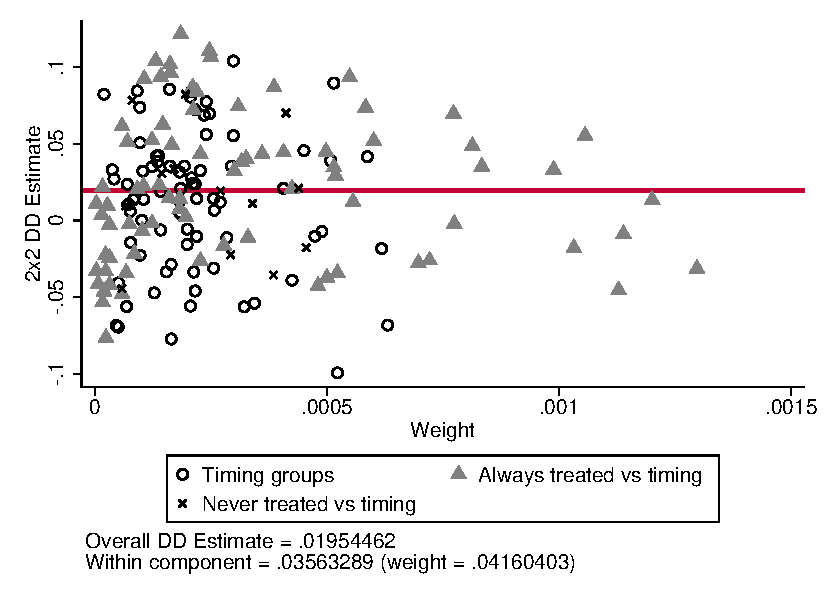
\includegraphics[width=0.85\textwidth]{figures/s12_bacon_decomposition.pdf}
    \caption*{\footnotesize \textit{Note: Decomposition of the TWFE DiD coefficient into timing-group comparisons following \citet{GoodmanBacon2021}. 95.4\% of weight comes from never-treated vs.\ timing comparisons.}}
\end{figure}

\autoref{fig:cs} reports the Callaway and Sant'Anna event study. The aggregated pre-treatment average is $0.0059$ with a standard error of $0.0020$ and a $p$-value of $0.002$. The post-treatment average is $0.0073$ with a standard error of $0.0070$ and a $p$-value of $0.299$. That positive pre-treatment average is in tension with the main event-study design. Because this implementation uses annual data, a balanced panel, no weights, and no controls, I treat it as a cautionary check rather than the preferred estimate.

% --- Figure A6: C&S Event Study ---
\begin{figure}[!htbp]
    \centering
    \caption{Callaway \& Sant'Anna Event Study}
    \label{fig:cs}
    \includegraphics[width=0.85\textwidth]{figures/s13_event_study_cs.pdf}
    \caption*{\footnotesize \textit{Note: Callaway and Sant'Anna DiD estimator following \citet{CallawaySantAnna2021}. Annual frequency, balanced panel, not-yet-treated and never-treated as controls. Cohorts restricted to 2009--2022.}}
\end{figure}

\autoref{fig:placebo} reports the unemployment placebo. The pre-trend test fails, with $F(3,338) = 7.22$ and $p = 0.0001$, so this figure should be read as a warning sign rather than supportive evidence. I keep it in the appendix because it is informative about the possibility of residual local dynamics around treatment timing.

% --- Figure A7: Placebo Event Study ---
\begin{figure}[!htbp]
    \centering
    \caption{Placebo Event Study: County Unemployment Rate}
    \label{fig:placebo}
    \includegraphics[width=0.85\textwidth]{figures/s14_event_study_placebo.pdf}
    \caption*{\footnotesize \textit{Note: Event-study coefficients with county unemployment rate as the dependent variable. Pre-trend F-test: $F(3, 338) = 7.22$, $p = 0.0001$.}}
\end{figure}
\FloatBarrier

Two additional diagnostics are not plotted here but still matter for interpretation. In the leave-one-out exercise, excluding Florida reduces the late-post-treatment estimate from about $-0.029$ to $-0.017$ and makes it statistically insignificant, while exclusions of other states leave the estimate close to the baseline value. Under state-level clustering, the $\tau{+}4$ coefficient remains $-0.0287$, and the standard error rises to $0.0132$, which yields a 95 percent confidence interval of $[-0.0545, -0.0029]$. Those checks do not reverse the sign of the main result, and state-level clustering preserves statistical significance.


\section{Data Construction Details}\label{app:data}

I begin the geographic construction with 33,782 ZIP codes from the SimpleMaps ZIP database and restrict the sample to 5,450 ZIP codes located in NOAA coastal counties. Then, I overlay FEMA's effective S\_LOMR polygons onto Census ZCTA boundaries to identify exposure to official map revisions. At the ZIP level, this procedure records the number of matched LOMRs, the first and last effective dates, and a geographic treatment-intensity measure equal to the overlap area between the LOMR polygon and the ZIP proxy geography divided by total ZIP area. In the full 5,450-ZIP coastal universe (before the Zillow coverage screen), the overlay yields 2,936 LOMR--ZIP pairs, 1,162 ever-treated ZIP codes, and 886 ZIP codes whose first observed LOMR falls inside the 2009--2022 window. After restricting to the 4,836 ZIP codes with usable Zillow data, those counts fall to 1,125 ever-treated and 855 first-in-window, as reported in \autoref{tab:sample_construction}.

I merge those treatment measures to monthly Zillow ZIP-level home values, county unemployment rates from BLS LAUS, and OpenFEMA NFIP policies and claims aggregated to the ZIP-month level. The NFIP aggregation yields policy counts, total premiums, average premiums, SFHA zone share, claims counts, and total claims paid. I deflate Zillow values to December 2022 dollars with the Consumer Price Index for All Urban Consumers. The merged monthly panel is then exported for estimation, where it is collapsed to quarters (averaging monthly log values within each quarter) because the ZHVI is already a three-month smoothed index. At the estimation stage, I winsorize the quarterly log home values at the 1st and 99th percentiles and impose the sample restrictions: I drop ZIP codes treated before 2009 and ZIP codes with multiple LOMRs. The resulting quarterly estimation sample contains 4,272 ZIP codes.

The heterogeneity variables require additional construction choices. I define policy intensity as the ZIP's pre-treatment average NFIP policy count divided by population, and I drop ZIP codes with values above one because those cases imply implausible denominators. I classify proxy upzoning and downzoning by comparing mean NFIP SFHA zone share in the 12 months before and after the LOMR effective date; ZIP codes with a change exceeding $\pm 1$ percentage point are classified as upzoned or downzoned, and the remainder as stable. This measure should be read as an exposure proxy rather than a direct parcel-level map transition. I construct the political heterogeneity measure from county-level mean Republican two-party vote share, split at the sample median, and I construct the disclosure variables from hand-coded state flood-disclosure rules. Those choices still shape the interpretation of the heterogeneity results, because each one trades cleaner coverage for a less direct measure of the underlying institutional channel.


\end{document}
